\documentclass{beamer}

\mode<presentation> {
\usetheme{bits}
%\setbeamertemplate{Fluid Mechanics} % To remove the footer line in all slides uncomment this line
% \setbeamertemplate{footline}{} % To replace the footer line in all slides with a simple slide count uncomment this line
\setbeamertemplate{navigation symbols}{} % To remove the navigation symbols from the bottom of all slides uncomment this line
}
\usepackage{graphicx} % Allows including images
\usepackage{booktabs} % Allows the use of \toprule, \midrule and \bottomrule in tables
\usepackage[english]{babel}
\usepackage{listings,multimedia}
\usepackage{multimedia}
\usepackage{ulem}
\usepackage{chemfig}
\usepackage{amsmath}
\usepackage{mathtools}
\usepackage{commath}
\usepackage{float}
\usepackage{caption}
\usepackage{multirow}
\usepackage{amssymb}
\usepackage{tikz}
\usepackage[labelformat=empty]{caption}
\usepackage{subfig}
\renewcommand{\thesubfigure}{}
\newcommand{\lmath}[1]{$\mathrm{#1}$}
\newcommand{\lbmath}[1]{$\mathbf{#1}$}

\usepackage{csquotes}
\usepackage[backend=biber]{biblatex}
\addbibresource{ref.bib}
\setbeamertemplate{bibliography item}{\insertbiblabel}

\newenvironment{descrsf}[1]
  {\begin{list}{}{\renewcommand{\makelabel}[1]{\textsf{##1}\hfil}
                  \setlength{\itemsep}{0.5em}
                  \setlength{\parsep}{0pt}
                  \settowidth{\labelwidth}{\textsf{#1}}
                  \setlength{\labelsep}{10pt}
                  \setlength{\leftmargin}{\labelwidth}
                  \addtolength{\leftmargin}{\labelsep}
                  \providecommand{\descriptionlabel}[1]%
                  {\hspace{\labelsep}\textsf{#1}}
                 }
  }
  {\end{list}}
  \newcommand\blfootnote[1]{%
  \begingroup
  \renewcommand\thefootnote{}\footnote{#1}%
  \addtocounter{footnote}{-1}%
  \endgroup
}

\newcommand{\addlogo}{\hfill\includegraphics[width=.2\textwidth,height=0.05\paperheight,trim=0 -0.65cm 1.5cm 2cm]{brand_strip_logo.png}}
\newcommand{\bitstitle}[1]{\makebox[\framewidth]{#1 \addlogo}}

%----------------------------------------------------------------------------------------
%	TITLE PAGE
%----------------------------------------------------------------------------------------
\usefonttheme{serif}
\title[Firmware verification for wBMS]{\small{Firmware verification for Automotive Wireless Battery Monitoring Systems \\[1ex]}} % The short title appears at the bottom of every slide, the full title is only on the title page
\author[Sai Kartik]{\begin{tabular}{r@{ }l} 
  Author:       & Sai Kartik (2020A3PS0435P) \\
  Manager:  & Mr. Abhinandan Subbarao\\
  Professor:    & Dr. Sathisha Shet K \\
  PS Station: & Analog Devices, India
\end{tabular}} % Your name
\institute[BPPC]{BITS Pilani, Pilani Campus} % Your institution as it will appear on the bottom of every slide, may be 
 \date{December 15,2023} % Date, can be changed to a custom date

\begin{document}
\setbeamertemplate{footline}{}
\begin{frame}
  \titlepage
\end{frame}

\begin{frame}
  \frametitle{\bitstitle{Outline}}
  \tableofcontents
\end{frame}

\setbeamertemplate{footline}[infolines theme]

\section{Aim and Problem statement}
\begin{frame}
  \frametitle{\bitstitle{Aim and Problem statement}}
  \textbf{Aim} \\ This project aims to verify the firmware of battery monitor sensors for a car's wireless battery monitoring system (wBMS).
  \vfill
  \textbf{Problem statement} \\ Use automation concepts to test the software and deliver it to customers quickly and efficiently without bugs.
\end{frame}

\section{Main Objectives}
\begin{frame}
  \frametitle{\bitstitle{Main Objectives}}
  \begin{itemize}
    \item To identify the testcases to be executed on wBMS system \pause
    \item To write scripts to perform manual testing of all tests \pause
    \item To automate the running of the test suite and generation of test report
  \end{itemize}

\end{frame}

\section{Design Methodologies}
\begin{frame}
  \frametitle{\bitstitle{Design Methodologies}}
  \begin{itemize}
    \item To perform manual testing, we flash the firmware onto the respective devices with JLink lite debuggers \pause \cite{ref40}
    \item Download files to the gateway and the nodes to facilitate communication between them \pause \cite{ref22}
    \item Configure the front-end application (GUI) to control the network and test the functionality. \pause
    \item Ensure the setup is RF-shielded fairly well
  \end{itemize}

\end{frame}

\section{Implementation}

\subsection{High level implementation}
\begin{frame}
  \frametitle{\bitstitle{High level implementation}}
  The software test cycle (STLC) mainly consists of 4 major steps to go through:
  \begin{itemize}
    \item Test planning \pause
    \item Test case development \pause
    \item Test environment setup \pause
    \item Test execution
  \end{itemize}

\end{frame}

\subsubsection{Test Planning}
\begin{frame}
  \frametitle{\bitstitle{Test Planning}}
  \begin{itemize}
    \item This step is the most significant part of software testing where the required testing strategies are created. \pause
    \item It is typically the team lead's/manager's role to establish the project cost and efforts required. \cite{ref32} \pause
    \item This phase begins once the requirement collection phase has been completed. \pause
    \item The major outcome of this phase is the finalised test plan/strategy which has to be adhered to.
  \end{itemize}

\end{frame}

\subsubsection{Test Case Development}
\begin{frame}
  \frametitle{\bitstitle{Test Case Development}}
  \begin{itemize}
    \item Once a strategy of the tests to be performed is outlined, the required data for it is gathered. \pause
    \item This data is organised to fit various test cases to ensure coverage of all possible scenarios. \pause
    \item Once the design of individual test cases is complete, each test case is linked in a chain in the Responsibility Traceability Matrix. \cite{ref33}
  \end{itemize}

\end{frame}

\subsubsection{Test environment setup}
\begin{frame}
  \frametitle{\bitstitle{Test Environment Setup}}
  \begin{itemize}
    \item This is a standalone task that is undertaken by the development team or the client to determine the environment the software is evaluated in. \pause
    \item The testing team should also come up with certain unit test cases to ensure the environment is ready.
  \end{itemize}

\end{frame}

\subsubsection{Test execution}
\begin{frame}
  \frametitle{\bitstitle{Test Execution}}
  \begin{itemize}
    \item In this phase, the testing team begins executing the test cases based on the strategy and environment decided. \pause
    \item If certain tests fail, the particular defect can be reported to the development team using a bug tracking system \pause
    \item Every failed test case should ideally be linked to at least one problem. This linking can help identify issues with the software \pause \cite{ref34}
    \item If a test case is blocked by a design flaw, they can be marked as such \pause
    \item A report consisting of all failed and blocked test cases can then be prepared and provided to the development team for them to take further action.
  \end{itemize}

\end{frame}

\subsection{Low Level implementation}

\begin{frame}
  \frametitle{\bitstitle{Low Level Implementation}}
  \begin{itemize}
    \item In order to exhaustively cover the testing of the software, there will be hundreds of test cases. \pause
    \item Maunally testing each case by using GUI elements is completely infeasible as it will consume a lot of time and human resources. \pause
    \item In order to overcome this issue, frameworks are built to test the software using various exposed API calls to the software. \pause
    \item As a major objective of this project, the frameworks are designed to be easily automated. \pause
    \item To allow everyone to access the test cases and modify them as necessary, open source software alternatives like pytest and python have been considered. \cite{pythondocs, pytest}%inser python, pytest refs
  \end{itemize}

\end{frame}

\subsubsection{Hardware setup}

\begin{frame}
  \frametitle{\bitstitle{Hardware Setup}}
  As discussed earlier, the gateways and nodes of the network are flashed with the software provided by the development team. \\
  The development boards housing the neessary components are equipped with the required hardware pins to allow quick flashing through internal applications developed by ADI. \\

  \begin{figure}
    \centering
    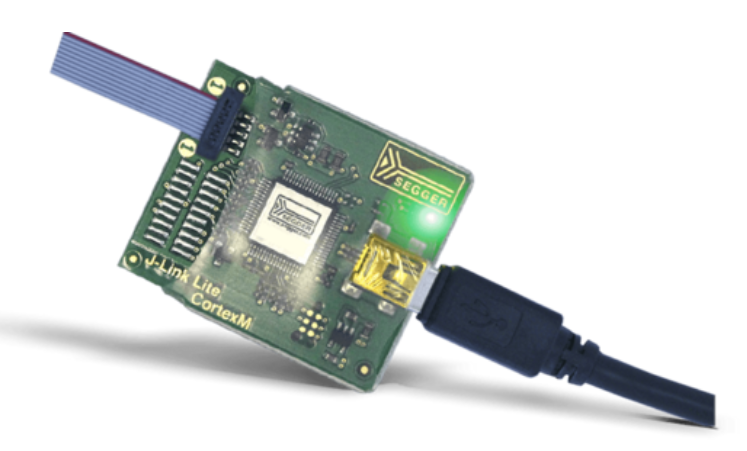
\includegraphics[scale=0.25]{figures/jlink.png}
    \caption*{J-link Lite debugger}
  \end{figure}

  Once the relevant firmware has been flashed onto the respective devices, the nodes are made to join the network created by the gateways

\end{frame}

\subsubsection{Software setup}

\begin{frame}
  \frametitle{\bitstitle{Software setup: Pytest framework}}
  Once the hardware is completely setup and the network is formed, the configuration for the devices in the network are uploaded to them through a GUI tool. This will ensure the reliance of the messages transmitted in the network. \\
  In order to allow automation, this tool can be designed to expose certain API endpoints which can be used by python scripts to communicate and carry tasks at a much faster pace compared to manual interaction with the GUI tool. \\

\end{frame}

\begin{frame}[allowframebreaks]
  \frametitle{\bitstitle{Software setup: Pytest framework}}
  To fast-track the process further in terms of validation and testing, we can use the pytest library along with certain packages that allow communication with the wireless network. \\
  Since this is a very popular framework, there are a lot of tools engineered to make our lives easy. This framework integrates easily with development applications such as VSCode and provides a clean user interface to the tests. \\

  \begin{figure}
    \centering
    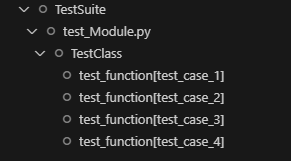
\includegraphics[scale=0.4]{figures/untested.png}
  \end{figure}
  \begin{figure}
    \centering
    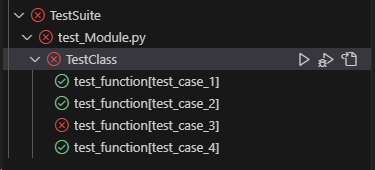
\includegraphics[scale=0.4]{figures/tested.png}
  \end{figure}

  The user can decide to run specific tests to test various functionalites of the system as and when needed. \\
  If we want to automate a larger batch of tests, we can use the command line options that pytest provides. This tool combined with a CI-CD tool like Jenkins to set triggers for various times to test \cite{jenkins}
\end{frame}

\section{Conclusion}

\begin{frame}
  \frametitle{\bitstitle{Conclusion}}
  We have seen how with the use of certain freely available tools along with standard industry practices, we were able to interface with a complicated wireless battery monitoring system and verify that the software complies with industry standards

\end{frame}

\setbeamertemplate{footline}{}
\begin{frame}[allowframebreaks]
  \frametitle{\bitstitle{References\footnote[frame]{Other documents regarding specific hardware/software architecture are for internal use only and cannot be shared as open sources/references}}}
  \tiny
  \printbibliography
\end{frame}

\end{document}